\documentclass{standalone}
\usepackage{tikz,tikz-cd}
\usetikzlibrary{calc, decorations.pathmorphing, decorations.markings, positioning, shapes, snakes, arrows, patterns, hobby, arrows.meta}
\newcommand{\zp}{\text{Z}^{\prime}}
\newcommand{\zpm}{\text{Z}^{\prime \mu}}
\tikzset{
>=triangle 45,
pos=.8,
scalar/.style={decorate, dashed, draw=blue},
photon/.style={decorate, thick,decoration={snake,segment length=5,post length=1mm,pre length = 1.5mm}},
boson/.style={decorate, thick,draw=blue,decoration={snake,segment length=5,post length=1mm,pre length = 1mm}},
particle/.style={draw=black, postaction={decorate}},
fermion/.style={draw=black, postaction={decorate}, decoration={markings,mark=at position .5 with {\arrow[draw=black,scale=1.5,>=stealth]{>}}}},
antifermion/.style={draw=black, postaction={decorate},decoration={markings,mark=at position .5 with {\arrow[draw=black,scale=1.5,>=stealth]{<}}}},
gluon/.style={decorate, draw=black,decoration={coil,amplitude=4pt, segment length=5pt}},
}
%-----------------------------------------------------------
%-----------------------------------------------------------
%-----------------------------------------------------------
\begin{document}

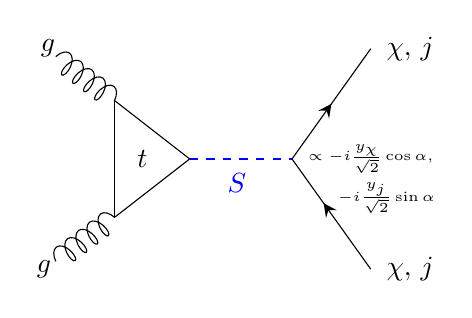
\begin{tikzpicture}    
    \node at (-0.1,2.9) {$g$};
    \node at (-0.15,0.1) {$g$};
    \node at (4.5,2.9) {$\chi,\, j$};
    \node at (4.5,0.1) {$\chi,\, j$};
    \draw[gluon] (0,2.8) to (0.8,2.2);
    \draw[gluon] (0, 0.2) to (0.8,0.8);
    \draw[particle] (0.75,2.23) to (0.75,0.75);
    \draw[particle] (0.8,0.8) to (1.7,1.5);
    \draw[particle] (0.8,2.2) to (1.7,1.5);
    \draw[scalar] (1.7,1.5) to (3,1.5);
    \node at (2.3,1.2) {\textcolor{blue}{$S$}};
    \draw[fermion] (3,1.5) to (4,2.9);
    \draw[antifermion] (3,1.5) to (4,0.1);
    %\draw[gluon] (2.,3) to  (1.22,1.86);
    %\node at (2.2,3.2) {$g$};
    %\node at (-0.2,1.5) {\scriptsize $ -i  \frac{y_{t}}{\sqrt{2}} \sin{\alpha}  \propto $};
    \node at (4.0,1.5) {\tiny $ \propto -i  \frac{y_{\chi}}{\sqrt{2}} \cos{\alpha} , $};
    \node at (4.2,1.0) {\tiny $ -i  \frac{y_{j}}{\sqrt{2}} \sin{\alpha} $};
    \node at (1.1,1.5) {$t$};
  \end{tikzpicture}
\end{document}